% V2: set-point and gain modification only.
% IEEE conference template (IEEEtran, conference mode), as in
% https://www.overleaf.com/latex/templates/ieee-conference-template/grfzhhncsfqn
\documentclass[conference]{IEEEtran}
\IEEEoverridecommandlockouts
\usepackage{cite}
\usepackage{amsmath,amssymb,amsfonts}
\usepackage{algorithm}
\usepackage{algorithmic}
\usepackage{graphicx}
\usepackage{textcomp}
\usepackage{xcolor}
\usepackage{booktabs}
\usepackage{url}
\usepackage{tikz}
\usetikzlibrary{arrows.meta,positioning,calc,fit}
\def\BibTeX{{\rm B\kern-.05em{\sc i\kern-.025em b}\kern-.08em
    T\kern-.1667em\lower.7ex\hbox{E}\kern-.125emX}}

\newcommand{\R}{\mathbb{R}}
\newcommand{\T}{^{\top}}
\newcommand{\mpc}{\mathrm{MPC}}
\newcommand{\xb}{\bar{x}}
\newcommand{\ub}{\bar{u}}
\newcommand{\zb}{\bar{z}}
\newcommand{\lb}{\bar{\lambda}}
\newcommand{\xh}{\hat{x}}
\DeclareMathOperator*{\argmin}{arg\,min}
\renewcommand{\algorithmicrequire}{\textbf{Input:}}
\renewcommand{\algorithmicensure}{\textbf{Output:}}
\begin{document}

\title{Residual Reinforcement Learning on the Feedback Policy of a Whole-Body MPC: Set-Point and Gain Modification for Humanoid Locomotion%
\thanks{Progress report. This work is carried out under the supervision of Prof.~Fumio Kanehiro and Dr.~Mehdi Benallegue.}}

\author{\IEEEauthorblockN{Norawit Nangsue}
% TODO(author): complete the affiliation and e-mail before submitting.
\IEEEauthorblockA{[Affiliation to be completed]}}

\maketitle

\begin{abstract}
Model predictive control (MPC) gives a humanoid robot a motion that respects its dynamics and constraints, but only as well as its model allows.
Reinforcement learning (RL) improves from experience, but an unstructured learned correction ignores everything the MPC already knows.
A whole-body MPC based on differential dynamic programming returns more than a torque trajectory: it returns a time-varying feedback policy, made of a state set-point and a gain matrix, that is executed between two solves.
This report proposes to place the learned residual on that feedback policy.
The RL policy shifts the set-point and modifies the gains, and the torque correction is produced by the MPC's own feedback law.
A set-point shift becomes a torque in the range of the Riccati gains, which is the first-order response of the MPC to a displaced state; a gain modification changes how the robot reacts to tracking errors without changing the nominal motion.
We give low-dimensional parametrizations of both that keep the correction consistent with the contacts and with the solver's local model: a contact-consistent set-point basis, gain scaling per joint or per state group, and a cost residual followed by one backward pass.
As the base controller, we implemented an intrinsically stable MPC gait generator with a reformulated footstep timing and position pre-optimization, feeding a whole-body MPC of the HRP-5P legs.
In MuJoCo simulation it walks at up to 0.3\,m/s with a mean whole-body solve time of 6.7\,ms, and recovers from 26 of 36 pushes.
Its failures define what the residual policy has to learn.
No residual policy has been trained yet; the experiments are specified but not run.
\end{abstract}

\begin{IEEEkeywords}
humanoid robots, legged locomotion, model predictive control, residual reinforcement learning, feedback gains
\end{IEEEkeywords}

% ======================================================================================================
\section{Introduction}

Two families of controllers now make humanoid robots walk.
The model-based family plans with a model: a reduced model such as the linear inverted pendulum (LIPM) \cite{kajita2001lipm,kajita2003preview} decides where the centre of mass (CoM) and the feet should go, and a whole-body controller, increasingly a whole-body MPC \cite{tassa2012synthesis,mastalli2020crocoddyl,dantec2022wbmpc}, turns that into joint torques.
The learning family trains a neural network policy in simulation with RL and transfers it to the robot \cite{hwangbo2019learning,lee2020learning,rudin2022minutes,radosavovic2024humanoid}.

Their strengths are complementary.
An MPC handles constraints explicitly and can be re-targeted without retraining, but its solution is optimal only for its model, and the model leaves out joint flexibility, contact compliance, actuator dynamics and the terms dropped to make the problem solvable in real time.
An RL policy absorbs such effects from experience and is robust in practice, but it is a black box whose behaviour is set at training time.

Residual RL \cite{silver2018residual,johannink2019residual} keeps the model-based controller and learns only a correction that is added to it.
The base controller makes exploration start from a working behaviour, and the policy only has to learn what the model misses.
Recent legged-robot results follow this pattern or a close variant \cite{gangapurwala2022rloc,kang2023rlmodel,jenelten2024dtc,cheng2025rambo,jeon2025residualmpc}.
In most of them the correction is added to the controller output, as a joint torque or a joint position target.
Such a correction is unstructured: it has one free number per joint at every control step, it is expressed in actuator coordinates, and nothing ties it to the model that produced the base action.

A whole-body MPC solved by differential dynamic programming (DDP) \cite{mayne1966ddp} offers a more structured place for the correction.
Along with the torque trajectory, the solver returns Riccati gains.
Together they form a feedback policy with two parts, a \emph{set-point} (the planned state) and a \emph{reactiveness} (the gains), which is the law that actually drives the robot between two solves \cite{grandia2019feedback,dantec2022firstorder,dantec2022wbmpc}.
This report studies residual RL on these two parts: the learned policy shifts the set-point and modifies the gains, and the MPC's feedback law converts both into torques.

The contributions of this progress report are:
\begin{itemize}
\item A formulation of residual RL on the DDP feedback policy (Section~\ref{sec:method}), with an analysis of what a set-point shift and a gain modification each do in closed loop.
\item Low-dimensional parametrizations of both: a contact-consistent set-point basis, and three gain parametrizations (output scaling, input scaling, cost residual) with their stability properties.
\item A base controller for the study (Section~\ref{sec:base}): an IS-MPC gait generator \cite{scianca2020ismpc} with footstep timing and position pre-optimization \cite{dallard2025adios}, for which we propose a scaled reformulation solved as a single nonlinear program, feeding a whole-body MPC of the HRP-5P \cite{kaneko2019hrp5p} legs built on Crocoddyl \cite{mastalli2020crocoddyl}.
\item Preliminary simulation results of the base controller (Section~\ref{sec:results}) that quantify its limits, and an experimental plan (Section~\ref{sec:plan}).
\end{itemize}

% ======================================================================================================
\section{Related Work}

\subsection{Gait generation with reduced models}
The zero-moment point (ZMP) \cite{vukobratovic2004zmp} and the LIPM \cite{kajita2001lipm} are the basis of preview control \cite{kajita2003preview} and of linear MPC gait generators, which later included the footsteps among the decision variables \cite{wieber2006mpc,herdt2010online}.
The unstable part of the LIPM is the divergent component of motion (DCM), also called the capture point \cite{pratt2006capture,takenaka2009dcm,englsberger2011capture}; capturability analysis \cite{koolen2012capturability} relates it to the number of steps needed to stop.
Lanari \emph{et al.} \cite{lanari2014boundedness} gave the condition under which the CoM stays bounded, and IS-MPC \cite{scianca2020ismpc} enforces this condition as a constraint.
Dallard \emph{et al.} \cite{dallard2025adios} closed the loop on the measured state and added a pre-optimization of footstep timing and position, as timing adaptation is essential for push recovery \cite{khadiv2020timing}.
Our base controller follows this line and the open-source implementation \cite{ismpcwalking}.

\subsection{Whole-body MPC and Riccati feedback}
DDP \cite{mayne1966ddp} and iLQR \cite{li2004ilqr} solve the whole-body optimal control problem fast enough for MPC \cite{tassa2012synthesis,mastalli2020crocoddyl}, and have been demonstrated on a torque-controlled humanoid \cite{dantec2022wbmpc}.
The backward pass returns time-varying feedback gains with the trajectory.
These Riccati gains are a first-order approximation of how the MPC solution changes with the state \cite{dantec2022firstorder}, and they are used to run the feedback at a higher rate than the solver \cite{grandia2019feedback,dantec2022wbmpc}.
Grandia \emph{et al.} \cite{grandia2019feedback} also showed that these gains must be consistent with the contact constraints to be usable on hardware.
The gains are optimal for the model, and in these works they are applied as computed; we propose to let a learned policy adjust them, and the set-point they act on, online.

\subsection{Reinforcement learning and its combination with MPC}
Policies trained with massively parallel simulation \cite{rudin2022minutes} and PPO \cite{schulman2017ppo} are now standard for legged robots \cite{hwangbo2019learning,lee2020learning,radosavovic2024humanoid}.
Model-based controllers enter this pipeline in several ways.
The policy can be asked to track a model-based plan, as in DTC \cite{jenelten2024dtc} or in on-demand optimal control references \cite{kang2023rlmodel}; it can output corrections to a model-based controller, as in RLOC \cite{gangapurwala2022rloc}, RAMBO \cite{cheng2025rambo} and Residual MPC \cite{jeon2025residualmpc}, the last of which adds torque residuals to a GPU-parallel whole-body MPC on a humanoid; or the MPC can be distilled into a network \cite{carius2020mpcnet,reske2021imitation}, which is fast but discards the online optimization.
In contrast to these works, our residual does not act on the output of the MPC but on the parameters of its feedback law.

\subsection{Learning gains and impedance}
Learning the gains of a controller instead of its output has a long history.
Variable impedance control learned with RL \cite{buchli2011variable} adapts joint stiffness along a motion, and the cost weights of an LQR have been tuned from data so that the resulting gains perform well on the real system \cite{marco2016lqr}.
RL has also been used to adjust the parameters of an MPC, by differentiating through the optimization \cite{amos2018diffmpc,romero2024acmpc} or by treating the MPC as a parametrized policy \cite{gros2020nmpcrl}.
We apply the idea to the time-varying gains of a whole-body MPC of a humanoid, online and at the rate of the solver's nodes, and combine it with a shift of the set-point.

% ======================================================================================================
\section{Base Controller}
\label{sec:base}

\begin{figure*}[t]
\centering
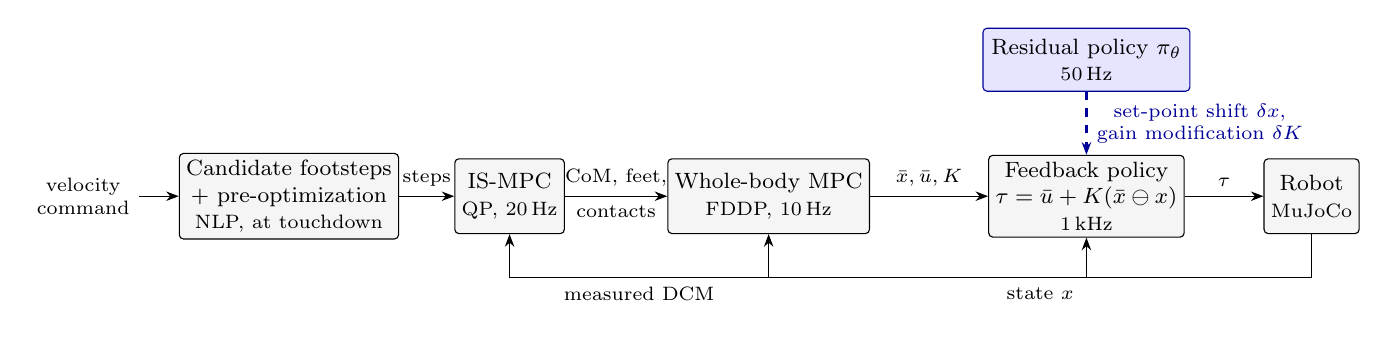
\begin{tikzpicture}[font=\footnotesize, >={Stealth[length=1.6mm]},
  blk/.style={draw, rounded corners=1.5pt, minimum height=9.5mm, align=center, inner sep=2.5pt, fill=black!4},
  res/.style={draw, rounded corners=1.5pt, minimum height=8mm, align=center, inner sep=3pt, fill=blue!10, draw=blue!60!black},
  lab/.style={font=\scriptsize, align=center},
  inj/.style={->, dashed, blue!60!black, thick}]
\node[lab] (cmd) {velocity\\command};
\node[blk, right=5mm of cmd] (ftpp) {Candidate footsteps\\+ pre-optimization\\{\scriptsize NLP, at touchdown}};
\node[blk, right=7mm of ftpp] (ismpc) {IS-MPC\\{\scriptsize QP, 20\,Hz}};
\node[blk, right=13mm of ismpc] (wb) {Whole-body MPC\\{\scriptsize FDDP, 10\,Hz}};
\node[blk, right=15mm of wb] (ric) {Feedback policy\\$\tau=\ub+K(\xb\ominus x)$\\{\scriptsize 1\,kHz}};
\node[blk, right=10mm of ric] (rob) {Robot\\{\scriptsize MuJoCo}};
\draw[->] (cmd) -- (ftpp);
\draw[->] (ftpp) -- node[lab, above] {steps} (ismpc);
\draw[->] (ismpc) -- node[lab, above] {CoM, feet,} node[lab, below] {contacts} (wb);
\draw[->] (wb) -- node[lab, above] {$\xb,\ub,K$} (ric);
\draw[->] (ric) -- node[lab, above] {$\tau$} (rob);
\coordinate (fb) at ($(rob.south)+(0,-5.5mm)$);
\draw[->] (rob.south) -- (fb) -| node[lab, pos=0.25, below] {state $x$} (wb.south);
\draw[->] (fb -| ric.south) -- (ric.south);
\draw[->] (fb -| wb.south) -| node[lab, pos=0.25, below] {measured DCM} (ismpc.south);
\node[res, above=8mm of ric] (pol) {Residual policy $\pi_\theta$\\{\scriptsize 50\,Hz}};
\draw[inj] (pol.south) -- node[lab, right, text=blue!60!black] {set-point shift $\delta x$,\\gain modification $\delta K$} (ric.north);
\end{tikzpicture}
\caption{Base controller (grey) and the proposed residual (blue, dashed). The whole-body MPC returns a feedback policy made of a set-point $\xb$, a feedforward torque $\ub$ and Riccati gains $K$. The residual policy shifts the set-point and modifies the gains; it never outputs a torque directly. Only the base controller is implemented so far.}
\label{fig:arch}
\end{figure*}

Fig.~\ref{fig:arch} shows the controller.
A gait generator based on the LIPM runs at 20\,Hz and produces CoM, foot and contact references; a whole-body MPC of the legs tracks them at 10\,Hz; its feedback policy is evaluated at 1\,kHz.

\subsection{LIPM and the stability condition}
With CoM position $c\in\R^2$, ZMP $p$ and $\eta=\sqrt{g/z_c}$ for a constant CoM height $z_c$, the LIPM is $\ddot c=\eta^2(c-p)$.
The DCM $\xi=c+\dot c/\eta$ splits it into a stable and an unstable first-order system,
\begin{equation}
\dot c=\eta(\xi-c),\qquad \dot\xi=\eta(\xi-p).
\label{eq:dcm}
\end{equation}
The CoM follows the DCM, and the DCM diverges from the ZMP.
The DCM stays bounded if and only if \cite{lanari2014boundedness}
\begin{equation}
\xi(t_0)=\eta\int_{0}^{\infty}e^{-\eta\tau}\,p(t_0+\tau)\,d\tau .
\label{eq:stab}
\end{equation}
The initial DCM cannot be chosen, so \eqref{eq:stab} is a constraint on the future ZMP trajectory.
IS-MPC \cite{scianca2020ismpc} enforces it while keeping the ZMP in the support polygon, by moving both the ZMP and the footsteps.

\subsection{Footstep timing and position pre-optimization}
After a push, \eqref{eq:stab} may have no solution with the nominal step times.
The pre-optimization of \cite{dallard2025adios} therefore adjusts the step positions $p_f^k$ and times $t_k$ before the MPC runs.
If the ZMP stays in the support region for all future times, integrating \eqref{eq:stab} piecewise over the steps shows that the initial DCM must lie in a time-weighted sum of the support regions.
With $\mu_k=e^{-\eta t_k}$ and $\Delta\mu_k=\mu_k-\mu_{k+1}$, the centre and half-size of this set are
\begin{equation}
c_\mu=\sum_{k=0}^{N_s-1}p_f^k\,\Delta\mu_k+p_f^{\mathrm{end}}\mu_{N_s},\quad
h_\mu=\sum_{k=0}^{N_s-1}\tfrac{d_k}{2}\,\Delta\mu_k+\tfrac{d}{2}\mu_{N_s},
\label{eq:ch}
\end{equation}
and the condition reads, in the frame $R$ of the support foot,
\begin{equation}
-h_\mu\le R\T\big(\xi(t_0)-c_\mu\big)+s\le h_\mu ,
\label{eq:ftpp}
\end{equation}
with a slack $s$ that is zero when the condition can be met.
Double support is sampled with the region moving linearly between the two feet, and all footsteps after the current one use the square inscribed in the sole ($d_k=d_y/\sqrt2$), so that \eqref{eq:ftpp} does not depend on their orientation.
Kinematic limits bound each step relative to the previous one, and timing constraints keep the phases ordered and within minimum and maximum durations.

The cost of \cite{dallard2025adios} penalizes the deviation from the nominal timing, the slack, and the footstep displacement weighted by a ratio of the form $(\Delta\mu_i)^2/(\Delta\hat\mu_i)^2$, where the hat denotes nominal values.
Two points make this problem awkward.
The variables $\mu_k$ decay exponentially with time and reach $10^{-7}$ at the end of a 5\,s preview, so the problem is badly scaled.
The reference implementation \cite{ismpcwalking} solves it by block coordinate descent, alternating twice between positions and times with a QP solver, and drops the divisor of the ratio.

We replace the decision variable $\mu_k$ by the ratio $\nu_k=\mu_k/\hat\mu_k$, which equals one when the timing is nominal.
The cost becomes
\begin{multline}
J=\sum_k(\nu_k-1)^2+w_s\|s\|^2\\
+K_s\sum_{i\ge1}\big\|p_f^i-\hat p_f^i\big\|^2\,
\frac{(\nu_i\hat\mu_i-\nu_{i-1}\hat\mu_{i-1})^2}{(\hat\mu_i-\hat\mu_{i-1})^2},
\label{eq:cost}
\end{multline}
all variables are of order one, and the ratio is kept as in the original formulation.
We solve positions and times jointly as one nonlinear program with CasADi \cite{andersson2019casadi} and IPOPT \cite{wachter2006ipopt}.
The program is built once per number of steps and cached, with the state, candidates and nominal timing as parameters, so a replan only runs the solver.

\subsection{IS-MPC}
The QP of IS-MPC takes the pre-optimized steps as candidates.
Its variables are the ZMP velocities $\dot p_j$ over a control horizon $T_c=2.5$\,s sampled at $\delta=50$\,ms and the footstep positions in that horizon.
It minimizes
\begin{equation}
\sum_j\|\dot p_j\|^2+\beta\sum_k\|p_f^k-\hat p_f^k\|^2+\gamma\sum_j\|p_j-\sigma_j\|^2 ,
\end{equation}
where $\sigma_j$ is the centre of the support region at sample $j$, subject to the ZMP lying in the (moving) support region, the kinematic limits, and the discrete form of \eqref{eq:stab},
\begin{equation}
\sum_{j=0}^{N_t-1}e^{-j\eta\delta}\dot p_j+\mathrm{tail}(p_f)=\frac{\eta}{1-e^{-\eta\delta}}\big(\xi_0-p_0\big).
\label{eq:stabqp}
\end{equation}
The tail is the anticipative tail of \cite{scianca2020ismpc}: beyond $T_c$ the ZMP is conjectured to follow the remaining pre-optimized steps up to the preview horizon $T_p=6$\,s and to stop at the midpoint of the last two feet.
The centring term ($\gamma$) keeps the ZMP away from the sole edges and leaves the problem a convex QP because $\sigma_j$ is linear in the footsteps.
The QP is assembled directly as sparse matrices and solved with OSQP \cite{stellato2020osqp}.

The generator replans (pre-optimization and QP) at every touchdown and re-solves the QP with fixed steps at every 50\,ms tick.
It also contains a velocity gate, a two-step stop, capture steps when the DCM leaves the support region while standing, and a DCM feedback law for standing.
A push is detected when the difference between the measured and the planned DCM jumps by more than 4\,cm within one tick; the gait state is then reset to the measured one.
The whole gait generator is about 750 lines of Python.

\subsection{Whole-body MPC and its feedback policy}
\label{sec:wb}
The whole-body optimal control problem uses the floating base and the twelve leg joints of HRP-5P ($n_v=18$); the upper body is held by a separate joint-space LQR and inverse dynamics.
The horizon has $H=25$ nodes of 20\,ms.
Contacts are rigid 6D constraints that follow the contact schedule of the gait generator, and the cost tracks the CoM and foot references with posture and torque regularization.
The problem is solved with the FDDP solver of Crocoddyl \cite{mastalli2020crocoddyl}, using Pinocchio \cite{carpentier2019pinocchio} for the dynamics, every 100\,ms with at most ten warm-started iterations.

The solve at time $k$ returns the state and torque trajectories and the Riccati gains, $\{\xb_{i|k},\ub_{i|k},K_{i|k}\}_{i=0}^{H}$.
Between solves, the torque is
\begin{equation}
\tau=\ub_{i|k}+K_{i|k}\,(\xb_{i|k}\ominus x),
\label{eq:riccati}
\end{equation}
evaluated at 1\,kHz with the measured state $x$ and the plan interpolated in time; $\ominus$ is the difference on the state manifold.
We write $\tau^{\mpc}$ for \eqref{eq:riccati} in the following.


% ======================================================================================================
\section{Set-Point and Gain Modification}
\label{sec:method}

\subsection{The feedback policy as the interface}
The law \eqref{eq:riccati} has two parts with different roles.
The set-point $\xb$ says where the robot should be; the gain $K$ says how strongly, and through which joints, it reacts when it is not there.
With the state ordered as base pose, joint positions, base velocity and joint velocities, the gain of the leg model is
\begin{equation}
K=\begin{bmatrix}K_{b}&K_{j}&K_{\dot b}&K_{\dot j}\end{bmatrix}\in\R^{12\times36},
\label{eq:kpart}
\end{equation}
with blocks of 6, 12, 6 and 12 columns.
$K_j$ and $K_{\dot j}$ play the role of a joint stiffness and damping, but they are full matrices that couple the joints.
$K_b$ and $K_{\dot b}$ have no equivalent in a joint-space controller: they map an error of the unactuated floating base to coordinated leg torques, using the contact model of the optimal control problem.

The solver runs every 100\,ms and the torque is computed every 1\,ms, so 100 control steps are executed with each solution, and the feedback policy alone determines how the robot behaves during that interval.
The solution is optimal for the model.
On the real system, or in a simulator with compliant contacts, two things can be wrong with it: the set-point can be a state the robot should not be driven to (for example one that requires a contact moment the sole cannot transmit), and the gains can be too stiff or too soft for dynamics that the model ignores.
These are the two quantities we let the learned policy adjust.

\subsection{Modified feedback law}
The residual policy $\pi_\theta$ outputs a set-point shift $\delta x$ and a gain modification $\delta K$, and the torque becomes
\begin{align}
\tau&=\ub+(K+\delta K)\,\big((\xb\oplus\delta x)\ominus x\big)\nonumber\\
&\approx\tau^{\mpc}+\underbrace{K\,\delta x}_{\text{set-point}}+\underbrace{\delta K\,e}_{\text{gain}}+\delta K\,\delta x,
\label{eq:l2}
\end{align}
where $e=\xb\ominus x$ is the tracking error and the approximation is exact in a vector space.
The policy acts at the rate of the solver's nodes, 50\,Hz, so it takes five decisions per MPC solution, each applied for 20 control steps.
With $\delta x=0$ and $\delta K=0$ the controller is exactly the base controller.
The policy network is initialized to output zero, so training starts from the behaviour of Section~\ref{sec:results}.

\subsection{Set-point modification}
\subsubsection{What it does}
The term $K\delta x$ is a torque residual restricted to the range of $K$.
It has a direct interpretation.
The Riccati policy is the first-order expansion of the MPC solution with respect to the state \cite{dantec2022firstorder}, so $K\delta x$ is, to first order, the change of torque that the MPC itself would command if the robot were displaced by $-\delta x$.
The policy thus acts as a learned bias on the state seen by the controller, and the resulting torque respects the trade-offs encoded in the cost, the dynamics and the contact model, which a free torque residual does not.

Two practical consequences follow.
First, the action is expressed in state coordinates and not in actuator coordinates.
Through $K_b$, the policy can ask for a shift of the base, such as ``move the pelvis 1\,cm toward the stance foot'', and the gain distributes it over the joints of both legs.
A torque residual would have to learn this mapping, which changes with the contact phase.
Second, the shift enters a loop that is already closed.
Let $\zeta_i=x_i\ominus\xb_i$ be the deviation of the robot from the plan and $A_i,B_i$ the dynamics Jacobians along it.
To first order,
\begin{equation}
\zeta_{i+1}=(A_i-B_iK_i)\,\zeta_i+B_iK_i\,\delta x_i .
\label{eq:cl}
\end{equation}
The shift is an input to the closed-loop system $A_i-B_iK_i$, which the Riccati gains stabilize for the local model, so a bounded shift produces a bounded deviation.
The robot does not move by $\delta x$ exactly: for a slowly varying shift it settles at $(I-A+BK)^{-1}BK\,\delta x$, close to $\delta x$ in the directions where the feedback dominates the open-loop dynamics and smaller elsewhere.

The shift acts only in the feedback law and is not sent to the solver.
The next solve starts from the measured state, which includes the effect of the shift, and by the first-order property above its first torque agrees with the Riccati policy at that state; the term $K\delta x$ is then added again.
A persistent correction therefore requires the policy to keep its output, which it can do since it runs faster than the solver.

\subsubsection{Parametrization}
A free $\delta x$ has 36 components, and most of them should not be used.
A shift of the stance-leg joints that moves the stance foot produces torques that fight the contact and only create internal forces.
We restrict the shift to configurations and make it consistent with the contacts:
\begin{equation}
\delta x=\begin{bmatrix}P_c\,S\,a_x\\ 0\end{bmatrix},\qquad P_c=I-J_c^{+}J_c ,
\label{eq:setpoint}
\end{equation}
where $a_x$ is the policy output, $S$ a selection matrix, $J_c$ the Jacobian of the feet in contact at that node and $J_c^{+}$ its pseudo-inverse.
The projector $P_c$ keeps the stance feet where the plan has them.
It leaves 12 free directions in single support and 6 in double support.
The velocity part of the set-point is not shifted.
We consider two choices of $S$:
\begin{itemize}
\item \emph{Base shift} (6 numbers): the policy outputs a change of the base pose, and the projection completes the leg joints so that the stance feet do not move. In double support this spans all admissible shifts.
\item \emph{Full shift} (18 numbers): base pose and leg joints, which adds the swing leg in single support.
\end{itemize}
The output is bounded twice: $a_x$ is clipped to a box (a few centimetres and degrees), and the resulting torque $K\delta x$ is clipped to a fraction of the joint torque limits, so that a large gain cannot turn a small shift into a large torque.

\subsection{Gain modification}
\subsubsection{What it does}
The term $\delta K\,e$ in \eqref{eq:l2} is bilinear in the policy output and the tracking error.
Without a tracking error it vanishes: a gain modification does not change the nominal motion, only the reaction to a disturbance.
It is the natural correction when the motion is right but the reaction is wrong, for example gains computed for a rigid contact that are too stiff for a compliant one, gains computed for a contact phase that has not started yet because the foot touched down late, or a reaction to a push that asks the ankle for more moment than the sole can transmit.

A free $\delta K$ is not practical.
The gain has $12\times36=432$ entries per node, and an arbitrary perturbation of them can destabilize the closed loop.
We consider three parametrizations with few parameters and known effects.

\subsubsection{Output scaling}
The gain is scaled on the torque side, per joint group:
\begin{equation}
K\leftarrow D_o\,K,\qquad D_o=\mathrm{diag}\big(e^{a_o}\big),
\label{eq:dout}
\end{equation}
with one parameter per group of joints (hip, knee and ankle of the stance and of the swing leg: 6 numbers).
It changes how much feedback torque each joint contributes, for example a softer ankle on the stance side.
The exponential keeps the scale positive, so a gain never changes sign.
This parametrization is the one for which classical robustness results apply: a continuous-time LQR with a diagonal input weight tolerates, in each input channel independently, a gain increase of any size and a reduction by half \cite{safonov1977margins}, and our control weight is diagonal.
The margins of a discrete, time-varying, finite-horizon gain are smaller, so the result indicates a direction and not a guarantee; the bounds on $a_o$ will be set empirically.

\subsubsection{Input scaling}
The gain is scaled on the error side, per state group:
\begin{equation}
K\leftarrow K\,D_i,\qquad D_i=\mathrm{diag}\big(e^{a_i}\big),
\end{equation}
with one parameter for each block of \eqref{eq:kpart} (4 numbers), optionally split between base position and orientation.
It changes how much the controller reacts to each kind of error: position against velocity, which is stiffness against damping, and base against joints.
It is equivalent to rescaling the error before the feedback and has no margin result, so its bounds are kept tighter.

\subsubsection{Cost residual}
The gains are a function of the cost.
Instead of modifying them directly, the policy modifies a few cost weights, $w\leftarrow w\,e^{a_w}$ (CoM, base orientation, feet, posture, torque), and the backward pass of the solver is run again along the current trajectory with the dynamics derivatives already computed.
Only the gains of this pass are used; the feedforward torque and the set-point are kept.
The new gains are optimal for a local problem with positive weights, so they are stabilizing for the local model by construction, and they remain coupled across joints as the original ones.
The price is one backward pass per policy decision.
A full solver iteration, which also computes the derivatives and a forward pass, takes about 0.8\,ms in our implementation (Section~\ref{sec:results}), which bounds this cost.

\subsubsection{Time variation}
A gain that changes quickly can destabilize a loop even when every frozen value is stabilizing.
The scale parameters are therefore low-pass filtered and rate-limited between policy decisions, and the policy is penalized for changing them.

\subsection{Summary of the action space}
Table~\ref{tab:param} lists the parametrizations.
The complete action is $a=(a_x,a_K)$ with between 10 and 28 numbers at 50\,Hz, against 12 numbers at the control rate for a torque residual, and every component has a physical meaning that can be bounded and inspected.
The correction is also limited: it cannot change the footsteps, the contact schedule or the feedforward torque.
Disturbances that require a different step remain the responsibility of the gait generator.

\begin{table}[t]
\caption{Parametrizations of the residual on the feedback policy}
\label{tab:param}
\centering
\setlength{\tabcolsep}{3pt}
\resizebox{\columnwidth}{!}{%
\begin{tabular}{@{}llcl@{}}
\toprule
 & Policy output & Size & Property\\
\midrule
\multicolumn{4}{@{}l}{\emph{Set-point} ($K\,\delta x$: changes the motion)}\\
Base shift & base pose, legs by projection & 6 & stance feet fixed\\
Full shift & base pose and leg joints & 18 & stance feet fixed\\
\midrule
\multicolumn{4}{@{}l}{\emph{Gain} ($\delta K\,e$: changes the reaction)}\\
Output scaling & scale per joint group & 6 & LQR margins \cite{safonov1977margins}\\
Input scaling & scale per state group & 4--5 & stiffness vs.\ damping\\
Cost residual & scale per cost weight & 5 & optimal for local model\\
\bottomrule
\end{tabular}}
\end{table}

\subsection{Learning setup}
\emph{Observation.} The measured state $x$; the tracking error $e$; the feedforward torque $\ub$; the contact flags and the phase of the step from the gait generator; the velocity command; the previous action.
The tracking error is given explicitly because the effect of a gain modification depends on it.

\emph{Reward.} Velocity tracking and staying upright, with penalties on the size and the rate of change of the action, on joint torques, on the measured centre of pressure approaching the sole edge, and on the tilt of a stance foot.
The last two target the failure modes observed in Section~\ref{sec:results}.

\emph{Training.} PPO \cite{schulman2017ppo} in simulation, with pushes, mass and friction randomization and command changes.
The MPC is part of the environment: no derivative of the solver is needed.

% ======================================================================================================
\section{Preliminary Results: Base Controller}
\label{sec:results}

No residual policy has been trained.
This section reports the base controller alone, to establish the baseline and to identify what the residual has to correct.

\subsection{Setup}
The HRP-5P model (59 degrees of freedom including the floating base, 104\,kg) is simulated in MuJoCo \cite{todorov2012mujoco} with a 1\,ms time step and torque control.
The LIPM height is the measured CoM height when the MPC starts ($z_c=1.014$\,m, $\eta=3.11$\,s$^{-1}$).
Steps last at most 0.8\,s, of which 85\,\% is single support, and the commands are limited to 0.3\,m/s forward and 0.3\,rad/s.
All runs are headless, on one thread of a laptop (Apple M5), with the controller computed inside the simulation loop, so computation time does not delay the control.
A run counts as a fall when the base drops below 0.5\,m.
Pushes are applied as an instantaneous change of the base velocity, $\Delta v=\eta\,d$, which shifts the DCM by $d$; for example, $d=0.08$\,m is 0.25\,m/s, an impulse of about 26\,N\,s.

\subsection{Walking}
Table~\ref{tab:walk} summarizes four commands, each applied for 5\,s (8\,s in the last row) and followed by a two-step stop.
The robot does not fall in any of them, and Fig.~\ref{fig:walk} shows the 0.3\,m/s run.
The measured DCM follows the planned one with an RMS error of 12 to 16\,mm, and the feet track their references within 31\,mm.
The whole-body solve takes 6.7\,ms on average and at most 14.2\,ms of the 100\,ms period, with 8.2 iterations on average.
A gait tick takes 2.2\,ms on average; a touchdown replan (pre-optimization and QP) takes 7.2\,ms on average and at most 11.9\,ms.
The first replan from standing takes 49\,ms, just within the 50\,ms tick.

\begin{table}[t]
\caption{Walking in simulation (base controller, no falls)}
\label{tab:walk}
\centering
\setlength{\tabcolsep}{3pt}
\resizebox{\columnwidth}{!}{%
\begin{tabular}{@{}lcccccc@{}}
\toprule
Command & Dist. & Steps & \multicolumn{2}{c}{Error (max) [mm]} & CoP & Solve [ms]\\
 & [m] & & foot & DCM & ratio$^{\mathrm a}$ & mean / max\\
\midrule
0.2\,m/s & 0.93 & 8 & 18 & 28 & 1.45 & 6.4 / 14.2\\
0.3\,m/s, 0.2\,rad/s & 1.46 & 9 & 31 & 40 & 1.81 & 6.9 / 10.0\\
$-0.15$\,m/s & 0.74 & 8 & 10 & 30 & 1.47 & 6.1 / 8.7\\
0.3\,m/s (8\,s) & 2.43 & 13 & 30 & 36 & 1.59 & 7.1 / 11.6\\
\bottomrule
\multicolumn{7}{@{}l}{$^{\mathrm a}$Largest measured CoP offset of a stance foot divided by the half-size}\\
\multicolumn{7}{@{}l}{\phantom{$^{\mathrm a}$}of the largest centred box inside the sole; above 1 is near the sole edge.}
\end{tabular}}
\end{table}

\begin{figure}[t]
\centering
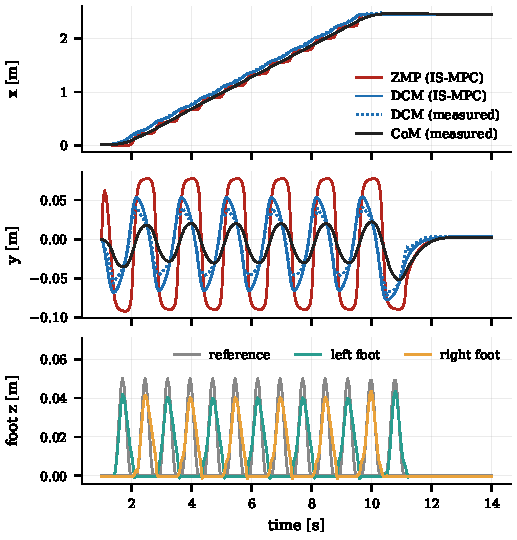
\includegraphics[width=\columnwidth]{figures/walk.pdf}
\caption{Walking at 0.3\,m/s for 8\,s, then stopping. Top and middle: ZMP and DCM planned by the IS-MPC, and DCM and CoM measured on the simulated robot. Bottom: foot height references and measured foot heights.}
\label{fig:walk}
\end{figure}

\subsection{Push recovery}
Table~\ref{tab:push} reports 36 pushes with the default settings: 20 while standing (five magnitudes, four directions) and 16 while walking at 0.2\,m/s (two magnitudes, four directions, two instants of the step cycle).
The robot stays up in 28 cases.
In two of them, lateral pushes of 0.10\,m while standing, it ends balanced on the edge of a foot tilted by 45$^\circ$, which we do not count as a recovery; this leaves 26 of 36.

\begin{table}[t]
\caption{Pushes survived, by DCM shift $d$ (four directions each)}
\label{tab:push}
\centering
\setlength{\tabcolsep}{4pt}
\begin{tabular}{@{}lcccccc@{}}
\toprule
\multicolumn{7}{@{}l}{\emph{Standing}}\\
$d$ [m] & 0.04 & 0.06 & 0.08 & 0.10 & 0.12 & Total\\
\midrule
Push detection on (default) & 4/4 & 4/4 & 4/4 & 1/4$^{\mathrm a}$ & 0/4 & 13/20\\
Push detection off & 4/4 & 4/4 & 2/4 & 1/4 & 0/4 & 11/20\\
\midrule
\multicolumn{7}{@{}l}{\emph{Walking at 0.2\,m/s} (two push instants)}\\
$d$ [m] & \multicolumn{2}{c}{0.05} & \multicolumn{2}{c}{0.08} & & Total\\
\midrule
Default & \multicolumn{2}{c}{7/8} & \multicolumn{2}{c}{6/8} & & 13/16\\
\bottomrule
\multicolumn{7}{@{}l}{$^{\mathrm a}$Two further cases stay up on a tilted foot and are not counted.}
\end{tabular}
\end{table}

\begin{figure}[t]
\centering
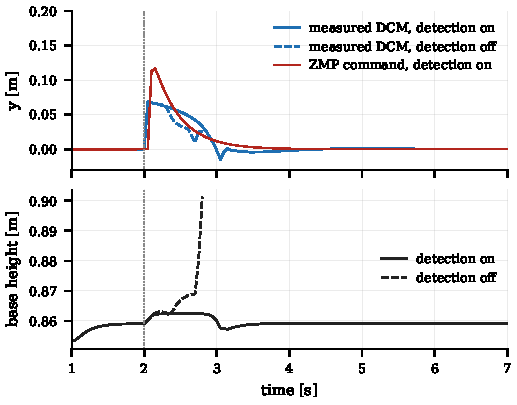
\includegraphics[width=\columnwidth]{figures/push.pdf}
\caption{Lateral push ($d=0.08$\,m, at 2\,s) while standing. With push detection, the gait state is reset to the measured DCM and the standing law moves the ZMP to bring it back. Without it, the whole-body MPC keeps tracking the unperturbed reference and the robot falls.}
\label{fig:push}
\end{figure}

Three observations follow.
First, closing the loop on the measured DCM helps while standing: with push detection, all pushes of 0.08\,m are recovered, against two of four without it (Fig.~\ref{fig:push}), and a forward push of 0.10\,m is recovered with a capture step.
Second, the failures are directional.
While walking, the three falls are all pushes toward the robot's right; while standing, the 0.10\,m failures are the backward push and the two lateral ones.
Third, in an earlier sweep with a previous parameter set, enabling push detection also during walking reduced the number of recovered pushes (17 of 24 against 21 of 24): resetting the reference to the pushed state removes the whole-body MPC's own pull toward the planned CoM.
Push detection is therefore active only while standing by default.


\subsection{What the residual has to correct}
The results point to three weaknesses, and each one maps to a part of the proposed residual.

\emph{Contact moments.} The CoP ratio in Table~\ref{tab:walk} exceeds 1 in every run, and after strong lateral pushes a stance foot rolls onto its edge.
The whole-body problem treats a stance foot as rigidly fixed, without a limit on the centre of pressure, so both its plan and its feedback ask for ankle moments that the sole cannot transmit.
Adding a wrench-cone penalty to the cost was tried and made walking fail with every weight large enough to change the plan, because the problem relies on these moments to track the lateral CoM reference.
A base set-point shift toward the stance foot reduces the moment the plan needs, and a lower output scale on the stance ankle reduces the moment the feedback asks for after a push.

\emph{Tracking lag.} The gait generator plans with the LIPM, and the robot lags its reference by 3 to 4\,cm of DCM in single support.
The lag is systematic and depends on the phase of the step, which is what a set-point shift that leads the reference can compensate.

\emph{Reaction to pushes.} The failures are directional, and the reaction that fails is the one computed by the Riccati gains for the unperturbed plan.
Whether a stiffer or a softer reaction would recover them, and in which state groups, is the question the gain modification is meant to answer.
Lateral step limits are narrow ($\pm3.5$\,cm around the nominal foot separation), so part of the lateral failures cannot be recovered without a different step and are outside the reach of this residual.

% ======================================================================================================
\section{Experimental Plan}
\label{sec:plan}

Table~\ref{tab:exp} lists the planned experiments.
Each one trains a policy with one parametrization of Table~\ref{tab:param} and evaluates it on the push protocol of Table~\ref{tab:push} and on the walking commands of Table~\ref{tab:walk}.
We plan to use mjlab \cite{zakka2026mjlab} so that training and the present MuJoCo evaluation share one physics engine.

\begin{table}[t]
\caption{Planned experiments}
\label{tab:exp}
\centering
\setlength{\tabcolsep}{3pt}
\begin{tabular}{@{}cp{0.36\columnwidth}p{0.47\columnwidth}@{}}
\toprule
 & Experiment & Question\\
\midrule
B0 & Base controller & Baseline (Section~\ref{sec:results}).\\
B1 & Torque residual with the same torque bound & Does the structure help, compared with an unstructured residual?\\
1 & Set-point, base shift & Does a 6-dimensional shift reduce the CoP ratio and the tracking lag?\\
2 & Set-point, full shift & What does the swing leg add?\\
3 & Gain, output scaling & Which joints should be softer or stiffer, and when?\\
4 & Gain, input scaling & Is the stiffness-to-damping ratio of the Riccati gains adequate?\\
5 & Gain, cost residual & Do gains that stay optimal for the local model perform better than scaled ones?\\
6 & Set-point and gain combined & Are the two corrections complementary?\\
\bottomrule
\end{tabular}
\end{table}

\emph{Metrics.} Pushes survived; velocity tracking; DCM error; CoP ratio and stance-foot tilt; size of the action and of the resulting torque correction; computation time.

\emph{Training cost.} The MPC runs on the CPU, so it bounds the training speed.
With the measured times, one simulated second costs about 67\,ms of whole-body solves and 44\,ms of gait ticks per environment.
At the 50\,Hz policy rate, $10^8$ policy steps are $2\times10^6$ simulated seconds, or about 60 core-hours of MPC, which is feasible on a CPU cluster without the GPU-parallel solver of \cite{jeon2025residualmpc}.
The cost residual adds at most one solver iteration per policy step, about 40\,ms per simulated second.

\emph{Open issues.} The bounds of each parametrization have to be found, starting from values at which the base behaviour is unchanged.
The state is taken from the simulator, and an estimator is required for the robot.
The controller must then be ported to mc\_rtc for experiments on HRP-5P.

% ======================================================================================================
\section{Conclusion}
This report proposed to place the residual of residual RL on the feedback policy that a DDP-based whole-body MPC returns, instead of on its output.
The learned policy shifts the set-point and modifies the gains.
A set-point shift becomes the torque the MPC would itself command for a displaced state and enters a loop that is already stabilized; a gain modification changes the reaction to tracking errors and leaves the nominal motion unchanged.
We gave parametrizations of both with 4 to 18 numbers, consistent with the contacts and, for the gains, with known stability properties.
The base controller needed for the study is implemented and walks in simulation, and its measured weaknesses map to the two parts of the residual.
The next step is to train the set-point and gain policies of Table~\ref{tab:exp} and compare them with an unstructured torque residual on the same push protocol.

\bibliographystyle{IEEEtran}
\bibliography{refs}

\end{document}
